\chapter{Methodology}
Here we describe the selected algorithms and their parameters in detail. We also discuss the nature of the benchmarks and real world data, giving a summary of the range of tests to be performed. The main goal of these tests is to provide a broader scope of network data to each approach than has been presented in literature thus far, to validate the effectiveness of each method at scale.

\section{Selected Algorithms}
\subsection{Tasgin-Bingol}
One of the earliest implementations of a genetic algorithm for the network clustering problem \cite{Tasgin2006}, Tasgin and Bingol's approach is an example of one of the more naive approaches. Each individual is represented as an array of size $n$, each index corresponding to a node of the input graph. The population is initialized by assigning each gene a random integer, bounded by the number of nodes in the graph. A subset of genes, the size of which is defined by a parameter referred to as the \textit{initialization rate} are selected, and propagate their community assignment to their neighbors. It utilizes modularity as its fitness function. Its mutation operator is simple. For the selected node $i$, select a member of $\Gamma(i)$, and set $i$ to be in its community.

\begin{table}[h!]
	\centering
	\begin{tabular}{|l | r| r|}
		\hline
		\multicolumn{1}{|c|}{\textbf{Parameter}} & \multicolumn{1}{|c|}{\textbf{Author's Default Value}}   & \multicolumn{1}{|c|}{\textbf{Selected Default Value}}\\
		\hline
		\hline
		Population Size & 100-250 & 300 \\
		\hline
		Generations & 200-500 & 30 \\
		\hline
		Elite Portion & Not reported & 0.10 \\
		\hline
		Mutation Rate & Not reported  & 0.10 \\
		\hline
		Initialization Rate & Not reported & 0.60 \\
		\hline
		Cleaning Rate & Not reported & 0.50 \\
		\hline
		Cleaning Threshold & Not reported & 0.70 \\
		\hline
		Cleaning Portion & Not reported & 0.50 \\ [0.2ex] 
		\hline
		
	\end{tabular}
	\caption{Parameters selected as the defaults for our implementation of Tasgin-Bingol's genetic algorithm for community detection, compared to the values reported by the authors}
	\label{table:tbgadef}
\end{table}
The authors describe a "one-way crossover", to tackle the main issue of the string of groups encoding; The same partition can be represented by multiple chromosomes. The crossover procedure is to randomly select a gene of the first parent, called the \textit{source}. The genes of the parent in this community are then copied to the second parent, the \textit{destination}, who lives on as the offspring. As mentioned in section 2, genetic operators on the string of groups representation can result in invalid partitions. This is addressed by another operation introduced by the authors, the \textit{cleanup} phase. In chapter 2, the concept of community variance is introduced. During the cleanup phase of the algorithm, some genes are randomly selected from a portion of individuals, and their community variance computed. If the community variance if above a parameter set by the user, that gene is assigned to the community most common to its neighbors.
The algorithm was tested by the authors on limited data, with very high parameters for generations and relatively small population sizes. After achieving results similar to those reported in\cite{Tasgin2006}, we choose to use a much more standard set of default parameters, shown in table \ref{table:tbgadef}. Our implementation uses roulette selection, as the authors left their chosen selection method ambiguous.

\subsection{GA-Net}

One of the most widely cited examples of a GA approach to network clustering, GA-Net\cite{Pizzuti2008} is an approach that seeks to optimize a score other than modularity, \textit{community score}, introduced in section 2.3. The individuals are represented using the locus adjacency representation. The initial population is generated randomly, with a guiding condition. When the gene for position $i$ is set to value $j$, a test for the existence of an edge between nodes $i$ and $j$ is performed. Each gene's set of possible alleles is limited to the nodes in its neighborhood. 

\begin{table}[h!]
	\centering
	\begin{tabular}{|l | r| r|}
		\hline
		\multicolumn{1}{|c|}{\textbf{Parameter}} & \multicolumn{1}{|c|}{\textbf{Selected Default Value}}\\
		\hline
		\hline
		Population Size &  300 \\
		\hline
		Generations &  30 \\
		\hline
		Elite Portion & 0.10 \\
		\hline
		Crossover Rate & 0.80 \\
		\hline
		Mutation Rate & 0.10 \\
		\hline
		Power Value & 1.5 \\ [0.2ex] 
		\hline
	\end{tabular}
	\caption{Parameters selected as the defaults for our implementation of GA-Net}
	\label{table:ganetdef}
\end{table}

The community score fitness function introduced in the paper aims to treat the community detection problem as finding a partition of a graph into $k$ subgraphs of maximum density, where $k$ is not known. Given a graph $G$, with adjacency matrix $A$, let $S=(I, J)$ be a sub-matrix of $A$, with $I$ being the subset of rows and $J$ being the subset of columns of $A$. Let $a_{iJ}$ be the mean value of the $i$th row, and $a_{Ij}$ be the mean of the $j$th column of $S$


\begin{align*}
a_{iJ}=\dfrac{1}{|J|}\Sigma_{j\in J}a_{ij}\nonumber \quad\text{and}\quad 
a_{Ij}=\dfrac{1}{|I|}\Sigma_{i\in I}a_{ij}
\end{align*}

The \textit{volume} of a graph, recall from section 2, is the total number of edges. Thus the volume of a submatrix $S = (I, J)$ is the number of connections between nodes of $S$. The power mean of $S$ of order $r$, $\mathbf{M}(S)$ is  
\begin{align*}
\mathbf{M}(S)=\dfrac{\Sigma_{i\in I}(a_{iJ})^r}{|I|}
\end{align*}

The \textit{score} of $S$ $Q(S)$ is defined as $\mathbf{M}(S)\times v_s$. Given a graph partitioned into communities, being a set of sub-matrices  $\{S_1,\dots S_k\}$, the \textit{community score} of the partitioning is

\begin{align*}
CS=\sum\limits_{i}^{k}Q(S_i)
\end{align*}

As the size of $I$ increases, or as the number of internal links in communities decreases, the value $r$ plays the role of scaling the value of the sub-matrix. The authors found that raising this parameter helps GA-Net perform as the definition of communities becomes weaker.

GA-Net employs a variation of uniform crossover, where two parents are chosen via roulette selection. These parents, $A$ and $B$, each have a portion of their genes used to produce a single new offspring $C$. A random bit vector is created, with genes selected from A where the bit is 1, and genes selected from B when it is 0.

\begin{figure}[!htb]
	\begin{center}
		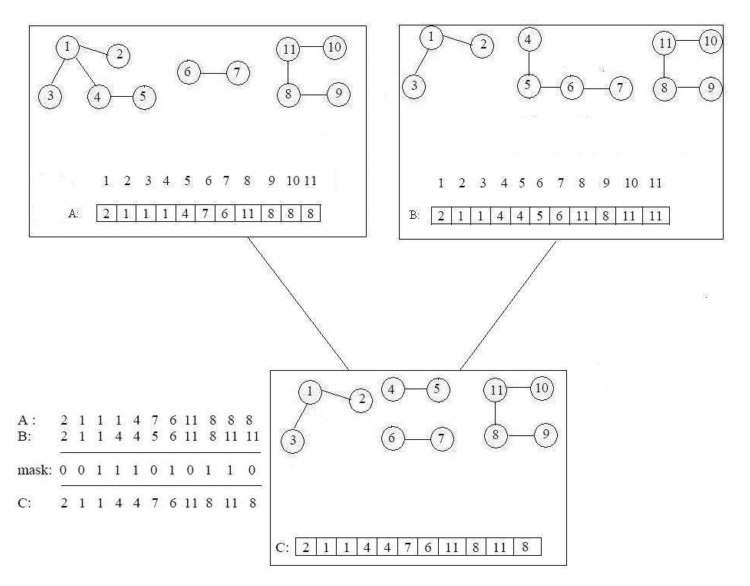
\includegraphics[scale=.8]{images/uni_graph.png}
	\end{center}
	\caption{An example of uniform crossover on two locus adjacency chromosomes}
	\label{logo}
\end{figure}



\subsection{GACD}
\cite{Shi2009}



\subsection{GALS}
GALS\cite{liu2013genetic}


\section{The Girvan-Newman Benchmark}

Girvan and Newman introduce a benchmark which is a special case of the planted $\ell$-partition model\cite{Girvan2002}. The graph is generated by creating 128 nodes, divided into 4 equally sized communities. Each node has an expected degree of 16. By setting the expected $k_{in}$ and $k_{out}$, the difficulty of discerning the partition can be tuned. With an expected $k_{out} < 8$, the communities are strongly defined. It should be expected that a well defined method should discern the structure with a fair degree of accuracy. 

The GN benchmarks limited size makes it an excellent model candidate for testing algorithms in early stages for the ability to detect loosely connected communities, but may not demonstrate the performance of a method when the input data is scaled up\cite{Yang2016}.


\section{The LFR Benchmark}



\begin{table}[h!]
	\centering
	\begin{tabular}{ |l | l| } 
		\hline
		\multicolumn{1}{|c|}{\textbf{Parameter}} & \multicolumn{1}{|c|}{\textbf{Description}} \\
		\hline
		\hline
		$N$ & Nodes \\ 
		\hline
		$k$ & Average Degree \\ 
		\hline
		$max_k$ & Maximum Degree \\ 
		\hline	
		$mu$ & Mixing Parameter \\ 
		\hline
		$min_c$ & Minimum Community Size \\
		\hline
		$max_c$ & Maximum Community Size \\ 
		\hline
	\end{tabular}
		\caption{The parameters of the LFR benchmark generator}
		\label{table:lfrparams}
\end{table}

All synthetic networks were created using Andrea Lancichinetti's benchmark generation application.


\section{Clustering Quality Measures}
The goal of this analysis is to compare the performance of the selected algorithms on a sufficient variety of networks, with sufficient complexity. The collection of generated and real world networks has been selected to reflect other comparative studies, and to extend the observations made in the literature proposing the algorithms. These networks come with ground truth, describing the community structure as it was generated, in the case of the synthetic networks, or as it is generally accepted when using real world data.

When comparing the generated community partitions, we use several measures

\subsection{Variation of Information}
\cite{Marina2007}

\subsection{Normalized Mutual Information}
The Normalized Mutual Information (NMI) of a community partition 

$$I(A,B)=\dfrac{-2\Sigma_{i=1}^{c_A}\Sigma_{j=1}^{c_B}C_{ij}log(C_{ij}M/C_iC_j)}{\Sigma_{i=1}^{c_A}
	C_ilog(C_i/N)+\Sigma_{j=1}^{c_B}C_jlog(C_j/N)}$$

\subsection{Rand and Adjusted Rand Index}
\cite{rand1971}


\section{Comparing Performance}

